%% 情報学群実験第3,4(C)用のレポートテンプレート
%
\documentclass[a4j,titlepage]{jarticle}
%% プリアンブルここから
\usepackage[dvipdfmx]{graphicx}
\usepackage{url}
\usepackage{comment}
\usepackage{here}
%
\title{\huge 配達支援システム\\
		内部設計書}
\author{第0版\\
        ONO-Systems\\}
\date{\today}

%本文
\begin{document}
\maketitle

%目次
\tableofcontents
\clearpage


\section{開発対象のシステム概要}
本システムは,配達物の配達支援を行うシステムです.主な機能を以下に示します.
\begin{itemize}
\item 消費者への通知機能
\item 配達員の位置情報の表示機能
\item 消費者の受取選択結果のリアルタイム表示機能
\end{itemize}


\section{開発環境}
本システムの開発環境を以下に示します.
\begin{itemize}
\item Android アプリケーション\\
  Android Studio ver4.2 
\item サーバ\\
  AWS(AmazonWebService)
\item 開発言語\\
  Java,MySQL
\item 文書・コード管理\\
  GitHub
\end{itemize}


\section{動作環境}
\begin{itemize}
\item Android アプリケーション\\
  Android 4.2
\item サーバ\\
  AWS(AmazonWebService)
\end{itemize}


\section{コーディング規約}
本プロジェクトのプログラムは,以下の規則を遵守します.
\subsection{コンポーネントやクラスについて}
\begin{itemize}
\item UpperCamelCaseを利用する
\item Component名は最後につける(Activity,Fragment,TextAreaなど)
\item 本プロジェクトで頻繁に利用する名詞は以下の表を用いて命名する(表\ref{termTable}参照)
\begin{table}[htb]
\centering
\caption{本プロジェクトで利用する名詞の英単語表}
\label{termTable}
\begin{tabular}{|ll|}
\hline
内部設計書での名前 & 英単語      \\ \hline
アカウント保持者  & User     \\
消費者       & Customer \\
配達員       & Courier  \\
配達物       & Delivery \\ \hline
\end{tabular}
\end{table}
\end{itemize}

\subsection{変数の命名について}
\begin{itemize}
\item 命名には英語を用いる
\item 名前から役割が読み取れるように命名する
\item グローバル変数に用いる英単語は省略しない(String ⇒ Strなど)
\item LowerCamelCaseを利用する
\item 定数は全て大文字で表し,スネークケースで連結する
\item forやwhileのカウンタ変数には,i,j,kを用いる
\end{itemize}

\subsection{関数の命名について}
\begin{itemize}
\item 意味と英単語の対応付けを統一する(表\ref{namingTable})
\item 名前は動詞で始める
\item LowerCamelCaseを利用する
\begin{table}[htb]
\centering
\caption{命名に使う英単語表}
\label{namingTable}
\begin{tabular}{|lll|}
\hline
意味            & 英単語    & 例                    \\ \hline
真偽値を取得        & is     & \#isCreated          \\
値を代入          & set    & \#setDelivery        \\
引数を含むか判定      & has    & \#hasFragment        \\
特定の動作をしたときに動作 & on     & \#onClick            \\
新しく作る         & create & \#createSubActivity  \\
新しく作る         & new    & \#newDelivery        \\
更新            & update & \#updateDeliveryDate \\
サーバから情報を取得    & fetch  & \#fetchDeliveryList  \\ \hline
\end{tabular}
\end{table}
\end{itemize}

\subsection{コーディングについて}
\begin{itemize}
\item 字下げは半角スペース2つを用いる
\item マジックナンバーは使用しない
\item 安易にネット上のソースコードを利用しない
\item classやif,whileなどのブロック始点のブラケット('\{')は改行せずに,半角スペースを空けて記述する
\item 機能が完成したとき(Pull Requestsを出すとき)にデバッグ用のコードを残さない
\end{itemize}

\subsection{コメントについて}
\begin{itemize}
    \item 複雑な処理はコメントをつける
    \item メソッドにはコメントをつける
    \item TODO:など,コードの説明でないコメントはPullRequestsを出すときには消す
\end{itemize}

\section{ネットワーク設計}
本システムのネットワークは図\ref{fig:n_d}のように構成されます.

\begin{figure}[H]
 \begin{center}
  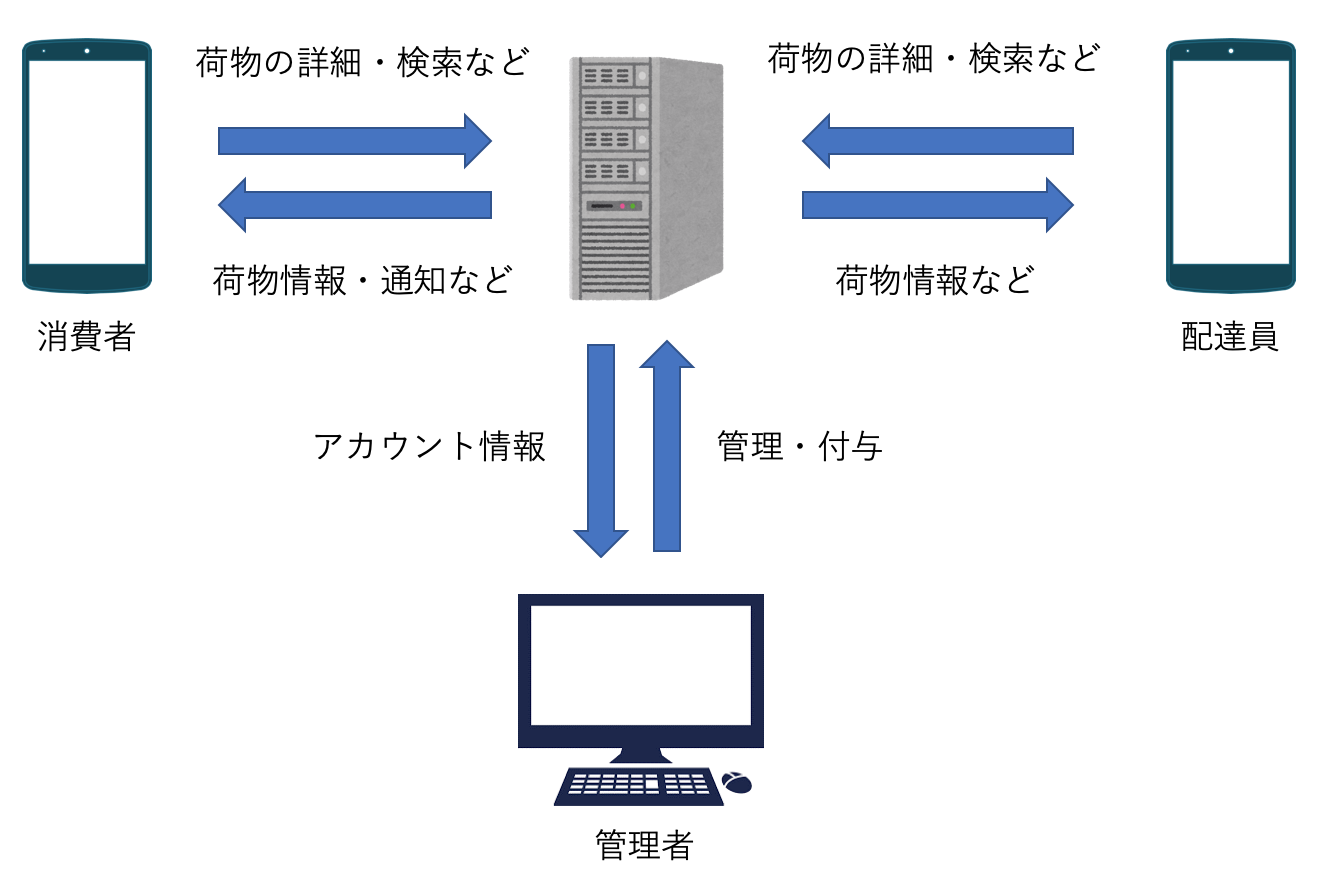
\includegraphics[width=140mm]{Network_Diagram.png}
  \caption{ネットワーク構成図}
  \label{fig:n_d}
 \end{center}

\end{figure}

\section{Android モジュール設計}
Androidのモジュール設計を以下に示します.
\subsection{モジュール構成}
本システムでの画面遷移は,図\ref{fig:login},\ref{fig:home}のようになっています.各画面を構成するモジュールについて説明します.
また,サーバとの通信に必要なモジュール,通知機能に関するモジュールなども設計します.
画面遷移する際は遷移先のモジュール呼び出しを行います.
本システムは消費者側と配達員側で遷移する画面が異なりますが,類似する機能が多数存在します.
そのため,共通部分は1つのモジュールとして作成し,異なる機能の実装は元となるモジュールを継承し消費者側と配達員側で分けて作成しています.
\begin{figure}[H]
 \begin{center}
  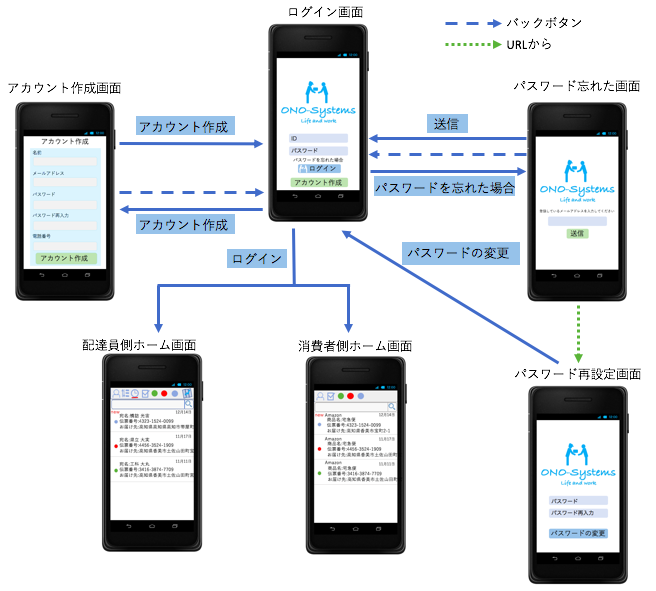
\includegraphics[width=150mm]{screen_transition_login.png}
  \caption{ログイン画面からの画面遷移図}
  \label{fig:login}
 \end{center}
\end{figure}
\begin{figure}[H]
 \begin{center}
  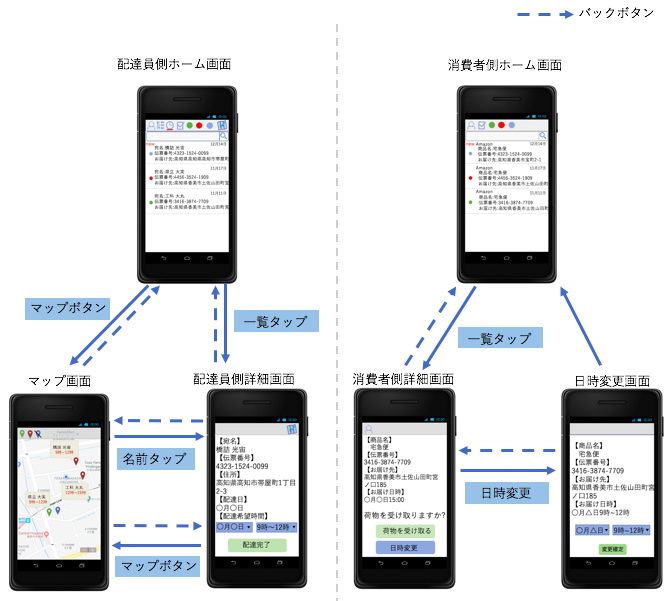
\includegraphics[width=150mm]{screen_transition_home.png}
  \caption{ホーム画面からの画面遷移図(左:配達員側,右:消費者側)}
  \label{fig:home}
 \end{center}
\end{figure}
\subsection{モジュール仕様}
Androidの各モジュールの仕様は以下の通りです.

\section{Server モジュール設計}
Serverのモジュール設計を以下に示します.
引数や返り値で使用している単語は,表\ref{serverTable}の通りです.
\begin{table}[htb]
\centering
\caption{本節で使用する変数の定義}
\label{serverTable}
\begin{tabular}{|lll|}
\hline
型 & 変数名 & 意味      \\ \hline
int & driver\verb|_|id & 配達員のID     \\
int & costomer\verb|_|id & 消費者のID     \\
string  & name  & 名前     \\
string & possword & パスワード     \\
string & mail & メールアドレス     \\
string & tel & 電話番号     \\
string & address & 住所     \\
long  &  slip\verb|_|number  & 伝票番号   \\
long & ship\verb|_|from & 発送元     \\
int & time & 配達日・時間     \\
int & receivable\verb|_|status & 配達状況    \\
int & deliveied\verb|_|status  &  受け取り可否  \\ \hline
\end{tabular}
\end{table}
receivable\verb|_|statusは,未配達を0,配達済みを1で表します.
deliveied\verb|_|statusは,未選択の状態を0,受け取れない場合は1,受け取れる場合は2で状態を表現します.

\subsection{モジュール構成}
サーバは,認証,配達員側,消費者側のモジュールに加え,管理者側や通知機能に関するモジュールから構成されています.

\subsection{モジュール仕様}
Serverの各モジュールの仕様は以下の通りです.
\subsubsection{認証機能}
ログインを行う際に使用する認証系のモジュールについて示します.
ログイン機能では,配達員側,消費者側どちらも同じモジュールを用いて認証を行います.
\begin{itemize}
\item Login.java\\
  動作: 初めにハッシュ値を計算しているか確認を行う.計算していなければパスワードからハッシュ値の計算を行いデータベースに値を格納する.次に,IDとパスワードからデータベースにあるハッシュ値を比較し,ログイン処理を行う.最後に,セッション情報をサーバ内に記憶させる.\\
  引数: id,password\\
  返り値: customer\verb|_|id,または,driver\verb|_|id,プラスuser\verb|_|type (NULL値なら認証不可)
\item AuthFilter.java\\
  動作: 認証が通っているかの判別を各サーブレットについて行う.判別にはセッション情報を用いる.このプログラムは,認証が必要な全てのサーブレットに対して行う.\\
  引数: なし\\
  返り値: なし
\item RegisterAccount.java\\
  動作: 入力された情報からデータベースに新たな消費者の登録を行う.また,パスワードからハッシュ値を計算しデータベース内に格納する.\\
  引数: name,mail,password,tel,address\\
  返り値: なし
\end{itemize}

\subsubsection{配達員側}
配達員側のモジュールを以下に示します.
\begin{itemize}
\item TopCourier.java\\
  動作: 当日に配達する荷物情報を,データベースからドライバーIDを参照して送信する.\\
  引数: driver\verb|_|id\\
  返り値: name,slip\verb|_|number,ship\verb|_|from,address,time,receivable\verb|_|status,deliveied\verb|_|status
\item SettingCourier.java\\
  動作: 配達員が入力した情報からデータベース内の配達員情報の変更を行う.\\
  引数: (配達員の)name,mail,password,tel\\
  返り値: なし
\item ChangeTimeCourier.java\\
  動作: 入力された情報からデータベース内の配達希望日時の変更を行う.\\
  引数: slip\verb|_|number,time\\
  返り値: time
\item CompleteCourier.java\\
  動作: 伝票番号からデータベース内の荷物情報に配達済みのフラグを立てる.\\
  引数: slip\verb|_|number\\
  返り値: なし
\item  InformationCourier.java\\
 動作: データベースから配達員の情報を取得し,送信する.\\
 引数: driver\verb|_|id\\
返り値: name,mail,tel
\end{itemize}

\subsubsection{消費者側}
消費者側のモジュールを以下に示します.
\begin{itemize}
\item TopCustomer.java\\
  動作: 入力された情報から利用者の荷物情報を送信する.\\
  引数: customer\verb|_|id\\
  返り値: name,slip\verb|_|number,ship\verb|_|from,address,time,receivable\verb|_|status,deliveied\verb|_|status
\item SettingCustomer.java\\
  動作: 入力された情報からデータベース内の消費者情報の変更を行う.\\
  引数: (消費者の)name,mail,password,tel,address\\
  返り値: なし
\item ReceiveCustomer.java\\
  動作: 伝票番号から荷物受け取りの可否をデータベース内に格納する.\\
  引数: slip\verb|_|number\\
  返り値: なし
\item ChangeTimeCustomer.java\\
  動作: 消費者が入力した情報からデータベース内の配達希望日時の変更を行う.\\
  引数: slip\verb|_|number,time\\
  返り値: time
  \item InformationCustomer.java\\
 動作: データベースから利用者の情報を取得し,送信する.\\
 引数: customer\verb|_|id\\
返り値: name,mail,tel,address
\end{itemize}

\subsubsection{通知機能}
通知機能のモジュールを以下に示します.
\begin{itemize}
\item Notification.java\\
  動作: トークンを受け取り,通知を送ってもらうようFirebaseに対してデータを送信する.\\
  引数: token\\
  返り値: token,text
\end{itemize}

\subsubsection{管理者側}
管理者側のモジュールを以下に示します.
\begin{itemize}
\item LoginManager.jsp\\
  動作: 管理者ページへのログインを行う.\\
  引数: id,password\\
  返り値: なし
\end{itemize}


\section{データベース設計}
本システムではデータベースにAWS(AmazonWebService)を使用します.\\
ER図など
\subsection{各テーブルの詳細}
本システムのデータベースには,5個のデータテーブルを用います.各データテーブルの役割と属性を以下に示します.
\subsubsection{消費者テーブル}
消費者テーブルでは,消費者に関する情報を管理します.このテーブルのデータテーブルを表\ref{customer}に示します.
\begin{table}[htb]
  \caption{消費者テーブル}
  \label{customer}
  \begin{center}
    \begin{tabular}{|c|c|c|c|c|c|} \hline
      属性 & データ型/長 & NULL & Key & 初期値 & その他 \\ \hline \hline
      customer\verb|_|id & int(9) unsigned & NO & PRIMARY & NULL & auto\verb|_|increment\\ \hline
      name & varchar(64) & NO &   &  & \\ \hline
      mail & varchar(64) & NO &   &  & \\ \hline
      tel & varchar(11) & YES &   & NULL & \\ \hline
      address & varchar(128) & YES &   & NULL & \\ \hline
      hash & varchar(255) & NO &   &  & \\ \hline
      salt & varchar(255) & NO &   &  & \\ \hline
    \end{tabular}
  \end{center}
\end{table}

\subsubsection{配達員テーブル}
配達員テーブルでは,配達員に関する情報を管理します.このテーブルのデータテーブルを表\ref{driver}に示します.
\begin{table}[htb]
  \caption{配達員テーブル}
  \label{driver}
  \begin{center}
    \begin{tabular}{|c|c|c|c|c|c|} \hline
      属性 & データ型/長 & NULL & Key & 初期値 & その他 \\ \hline \hline
      driver\verb|_|id & int(9) unsigned & NO & PRIMARY & NULL & auto\verb|_|increment\\ \hline
      name & varchar(64) & NO &   &  & \\ \hline
      mail & varchar(64) & NO &  &  & \\ \hline
      tel & varchar(11) & YES &  & NULL & \\ \hline
      store\verb|_|code & varchar(64) & YES &   & NULL & \\ \hline
      account\verb|_|type & int(1) unsigned & YES &   & NULL & \\ \hline
      hash & varchar(255) & NO &   &  & \\ \hline
      salt & varchar(255) & NO &   &  & \\ \hline
    \end{tabular}
  \end{center}
\end{table}

\subsubsection{商品テーブル}
商品テーブルでは,商品に関する情報を管理します.このテーブルのデータテーブルを表\ref{delivery}に示します.
\begin{table}[htb]
  \caption{商品テーブル}
  \label{delivery}
  \begin{center}
    \begin{tabular}{|c|c|c|c|c|c|} \hline
      属性 & データ型/長 & NULL & Key & 初期値 & その他 \\ \hline \hline
      slip\verb|_|number & varchar(12) & NO & PRIMARY & NULL & \\ \hline
      name & varchar(64) & NO &   &  & \\ \hline
      address & varchar(128) & NO &   &  & \\ \hline
      time & varchar(11) & YES &   & NULL & \\ \hline
      delivery\verb|_|status & int(1) unsigned & NO &   & 0 & \\ \hline
      receive\verb|_|status & int(1) unsigned & NO &  & 0 & \\ \hline
      customer\verb|_|id & int(9) unsigned & NO & MULTIPLE & NULL & \\ \hline
      driver\verb|_|id & int(9) unsigned & NO & MULTIPLE & NULL & \\ \hline
    \end{tabular}
  \end{center}
\end{table}

\subsubsection{管理者テーブル}
管理者テーブルでは,管理者に関する情報を管理します.このテーブルのデータテーブルを表\ref{manager}に示します.
\begin{table}[htb]
  \caption{管理者テーブル}
  \label{manager}
  \begin{center}
    \begin{tabular}{|c|c|c|c|c|c|} \hline
      属性 & データ型/長 & NULL & Key & 初期値 & その他 \\ \hline \hline
      manager\verb|_|id & int(1) unsigned & NO & PRIMARY & NULL & auto\verb|_|increment\\ \hline
      name & varchar(64) & NO &   &  & \\ \hline
      mail & varchar(64) & NO &  &  & \\ \hline
      store\verb|_|code & varchar(64) & YES &   & NULL & \\ \hline
      account\verb|_|type & int(1) unsigned & YES &   & NULL & \\ \hline
      hash & varchar(255) & NO &   &  & \\ \hline
      salt & varchar(255) & NO &   &  & \\ \hline
    \end{tabular}
  \end{center}
\end{table}

\subsubsection{地図テーブル}
地図テーブルでは,地図に関する情報を管理します.このテーブルのデータテーブルを表\ref{map}に示します.
\begin{table}[htb]
  \caption{地図テーブル}
  \label{map}
  \begin{center}
    \begin{tabular}{|c|c|c|c|c|c|} \hline
      属性 & データ型/長 & NULL & Key & 初期値 & その他 \\ \hline \hline
      map\verb|_|id & varchar(12) & NO & MULTIPLE & NULL & \\ \hline
      lat & double(8,6) & YES &   & NULL & \\ \hline
      lng & double(9,6) & YES &   & NULL & \\ \hline
    \end{tabular}
  \end{center}
\end{table}


\section{バージョン管理規約}
本システムの開発では,GitHub を用いてファイルの管理を行います.GitHub を使用する際には,以下の規則を遵守します.
\begin{itemize}
\item ドキュメント関連の資料は,onosystem-doc で管理する
\item Android のソースコードは,onosystem-android で管理する
\item Server のソースコードは,onosystem-server で管理する
\item 編集作業を行う際には,ブランチを切ってコミットする
\item 開発用ブランチの名前は,「dev\verb|_|○○(開発している機能名)」にする
\item 細かい頻度でコミットする(1日の作業ごとに纏めてコミットしない)
\item コミットのコメントはわかりやすい内容にする
\item Pull Requests されたものを確認し,評価をリアクションのアイコンを追加することで示す
\item Pull Requests に対して高評価が3つ以上ある場合には master に Merge する
\end{itemize}

\end{document}
